\chapter[Suporte Tecnológico]{Suporte Tecnológico}
\label{cap:suporte}

Este capítulo tem como principal objetivo apresentar as principais ferramentas e tecnologias 
a serem utilizadas na elaboração desse trabalho. De início, serão citadas as ferramentas 
relacionadas ao desenvolvimento, tais como o \textit{framework} Node.js e as ferramentas de 
virtualização de ambientes Docker e o Jest para desenvolvimento de testes automatizados. Em 
seguida serão apresentadas as ferramentas de apoio ao desenvolvimento, tais como o Firebase, 
uma plataforma de desenvolvimento de aplicativos móveis, oferecida pelo Google. O MongoDB, 
que é um sistema de gerenciamento de bancos de dados NoSQL (\textit{Not Only SQL}). O SonarQube, 
que é uma ferramenta de análise de qualidade código que nos possibilita ter acesso a diversas 
métricas. O GitHub, utilizado para o gerenciamento e armazenamento de código e, por fim, o 
Draw.io para elaboração de diagramas. 

\section{Ferramentas de Desenvolvimento}

\subsection{Node}

Como principal ferramenta de desenvolvimento \textit{back-end}, temos o Node \footnote{https://nodejs.org. Acessado pela última vez em 31/10/2023.} 
um \textit{framework} \textit{open-source} desenvolvido em JavaScript, que é bastante popular 
em soluções de grandes empresas como Netflix, LinkedIn, Uber, PayPal e Mozilla \cite{Kinsta}. 
Nesse cenário, é importante citar, também, o \textit{Express} \footnote{https://expressjs.com/. Acessado pela última vez em 31/10/2023.} 
que é um outro \textit{framework} \textit{open-source} construído em cima do Node e que 
simplifica o desenvolvimento de aplicações \textit{web} e APIs (Application Programming 
Interfaces), fornecendo uma camada de abastração sobre as funcionalidades básicas do Node.

Esse \textit{framework} tem como principais características, o seu roteamento que permite 
a definição de rotas para URLs específicas, facilitando seu mapeamento. A possibilidade de 
implementação de \textit{Middlewares} que são componentes ou funções que podem ser executadas 
em tempo de requisição HTTP, isso facilita a execução de tarefas como autenticação e validação. 

Além disso podemos citar algumas vantagens como o gerenciamento de requisições e respostas, 
o suporte aos vários métodos HTTP, a facilidade de integração, escalabilidade e desempenho, 
sua relevância no mercado atual e o tamanho da sua comunidade que acaba sendo de extrema 
importância para a evolução do \textit{framework}. 

\subsection{Jest}

O Jest \footnote{https://jestjs.io. Accesado pela última vez em 31/10/2023} é um \textit{framework} 
de testes automatizados amplamente utilizado na comunidade JavaScript principalmente em projetos 
do contexto de \textit{back-end} que utilizam Nest \footnote{https://nestjs.com. Acessado pela última vez em 31/10/2023.} 
e Node \footnote{https://nodejs.org. Acessado pela última vez em 31/10/2023.}. É uma ferramenta que 
foi desenvolvida pelo Facebook e visa facilitar o processo de escrita de testes unitários e de integração. 

Entre suas principais características, podemos citar sua facilidade de escrita onde os testes acabam 
ficando mais descritivos e legíveis, possibilidade de utilização de \textit{mocks} para simulação de 
resultados, retornos e comportamentos específicas, possibilidade de verificar a porcentagem de cobertura, 
tanto total do código, quanto total de cada arquivo individualmente, a fácil integração com ferramentas de 
CI e CD para a garantir que os testes sejam sempre executados quando houver uma alteração no código.

\subsection{Docker}

O Docker \footnote{https://www.docker.com. Accesado pela última vez em 31/10/2023} é uma ferramenta \textit{open-source} que visa facilitar o desenvolvimento, a execução e a 
implantação de um \textit{software} através de contêineres. Os contêineres são ambientes isolados, 
cujo todas as dependências do projeto estão nele empacotadas. Isso garante que, em todas as etapas, 
o ambiente seja o mesmo, isento de qualquer tipo de falha por incompatibilidade de versão ou algo 
do gênero.

Como principais características, podemos citar sua portabilidade, sua eficiência comparada 
às VMs, a facilidade de orquestração, a facilidade de subir um container de determinado \textit{framework} 
ou linguagem específica e a segurança e cofiabilidade empregada na implantação do Docker em um projeto.

\subsection{Firebase}

O Firebase\footnote{https://firebase.google.com. Accesado pela última vez em 31/10/2023} é um conjunto de serviços 
oferecidos pelo Google, no qual formam uma plataforma de desenvolvimento 
multiplataforma, que pode ser utilizada para criar aplicativos, jogos ou outros tipos de aplicações. 
O Firebase é uma plataforma \textit{Backend-as-a-Service} (BaaS), que basicamente 
oferece um back-end já pronto, ou seja, os desenvolvedores podem concentrar os esforços no front-end sem 
se preocupar em desenvolver e manter o back-end do produto \cite{AluraFirebase}.

Ao utilizar o Firebase, os desenvolvedores podem acelerar o processo de desenvolvimento de algumas
funcionalidades do projeto, por poder utilizar os recursos back-end já prontos da plataforma ao invés
de ter que desenvolvê-los. Além disso, o Firebase pode ser facilmente integrado a um projeto, por possuir 
SDKs (\textit{Software Development Kit}) em diversas linguagens de programação, e também oferece algumas funcionalidades que auxiliam no 
controle e melhoria da qualidade do produto \cite{AluraFirebase}.

\begin{figure}[h]
	\centering
	\caption{Produtos Oferecidos Pelo Firebase}
	\includegraphics[keepaspectratio=true,scale=1]{figuras/firebase-services.eps}
    \parbox{\linewidth}{\centering FONTE: \cite{RocketseatFirebase}}
	\label{fig-firebase-services}
\end{figure}

A Figura \ref{fig-firebase-services} ilustra alguns produtos oferecidos pelo Firebase que podem contribuir com as áreas de desenvolvimento, 
crescimento, análise de dados e geração de receita de uma aplicação. Os produtos são divididos em três categorias, 
sendo elas: criação, liberação e monitoramento e engajamento. Com isso, os desenvolvedores podem escolher os produtos baseado na 
funcionalidade que eles oferecem e na necessidade do projeto.

Dentre os produtos oferecidos pelo Firebase, vale destacar o Firebase Authentication, que tem o objetivo de facilitar e oferecer 
segurança na autenticação de usuários na aplicação. Além de oferecer suporte para a autenticação tradicional, que utiliza email, 
senha e telefone, ele também possibilita a autenticação por provedores de identidade como Google, Twitter, 
Facebook, Github e outros, sendo um modo de autenticação muito popular atualmente.

O Firebase oferece um plano gratuito, que permite a utilização livre da maioria de seus produtos até um certo limite de utilização. 
Quando este limite é ultrapassado, o plano deixa de ser gratuito, e os desenvolvedores podem escolher um dos planos pagos oferecidos 
baseado na necessidade e na escalabilidade da aplicação.

\subsection{MongoDB}

O MongoDB \footnote{https://www.mongodb.com. Accesado pela última vez em 31/10/2023} é um banco de dados NoSQL de código livre e orientado a documentos. 
Assim como se espera de um banco de dados NoSQL, 
o MongoDB possui uma alta flexibilidade no armazenamento de dados, que diferentemente de bancos de dados SQL, que armazenam dados 
em tabelas de linhas ou colunas, ele utiliza um formato chamado BSON, que é uma representação binária de dados. Com isso, as aplicações 
podem interagir com o banco de dados por meio do formato JSON, formato este que é muito utilizado atualmente. Um exemplo de um documento 
JSON descrevendo uma figura histórica pode ser vista na Figura \ref{fig-mongodb-json}.

\begin{figure}[h]
	\centering
	\caption{Exemplo de JSON em MongoDB}
	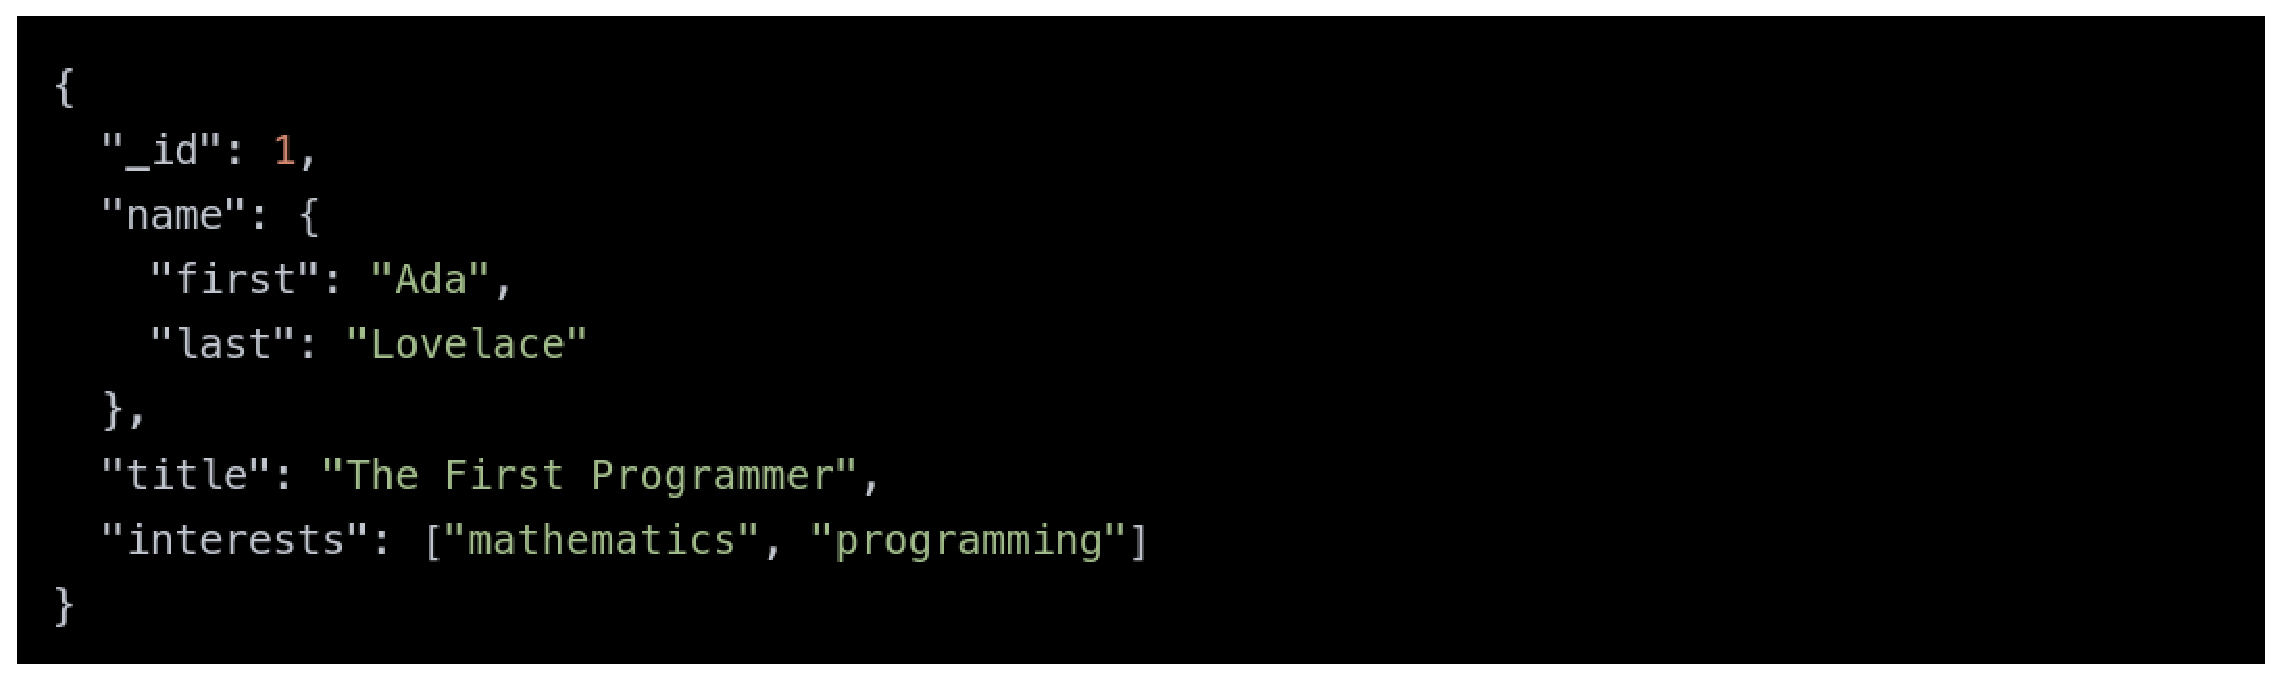
\includegraphics[keepaspectratio=true,scale=0.4]{figuras/mongodb-json.eps}
    \parbox{\linewidth}{\centering FONTE: \cite{MongoDB}}
	\label{fig-mongodb-json}
\end{figure}

Bancos de dados de documento são altamente flexíveis, o que permite que os documentos possam ser salvos parcialmente 
completos e também podendo ter diversas estruturas. Nos bancos de dados SQL, é possível realizar a indexação das colunas, 
para melhorar a performance nas operações do banco, o mesmo pode ser feito no MongoDB, mas ao invés de colunas, a indexação 
acontece nos campos do documento.

O MongoDB é muito popular atualmente, por possuir um fácil armazenamento de dados tanto estruturados como não estruturados, 
o que é possível por se tratar de um banco de dados de documentos. A possibilidade de armazenar os dados no formato JSON e por 
dispensar a necessidade de normalizar os dados também são propriedades muito atrativas para os desenvolvedores.

Além da flexibilidade no armazenamento, o MongoDB também possui uma arquitetura muito escalável, o que permite que pequenas máquinas 
trabalhem juntas para criar sistemas velozes e lidar com altos volumes de dados. Com isso, o MongoDB traz muitos benefícios para aplicações 
que precisam armazenar e interagir com uma alta carga de dados.

\subsection{SonarQube}

O SonarQube \footnote{https://docs.sonarsource.com/sonarqube/latest. Accesado pela última vez em 31/10/2023} é uma ferramenta auto 
gerenciável e automática de análise de código que ajuda na implementação das boas práticas de 
\textit{Clean Code} em um projeto de \textit{software}. Esta ferramenta pode ser inserida no \textit{workflow} de uma aplicação para 
gerar uma análise contínua de problemas no código fonte e sugestões de melhoria. O SonarQube possui suporte 
para uma grande variedade de linguagens de programação e pode ser integrada com \textit{pipelines} de CI e 
plataformas de DevOps, com o objetivo de garantir que a aplicação sempre esteja de acordo com os padrões de qualidade estabelecidos.

\begin{figure}[h]
	\centering
	\caption{SonarQube \textit{Workflow}}
	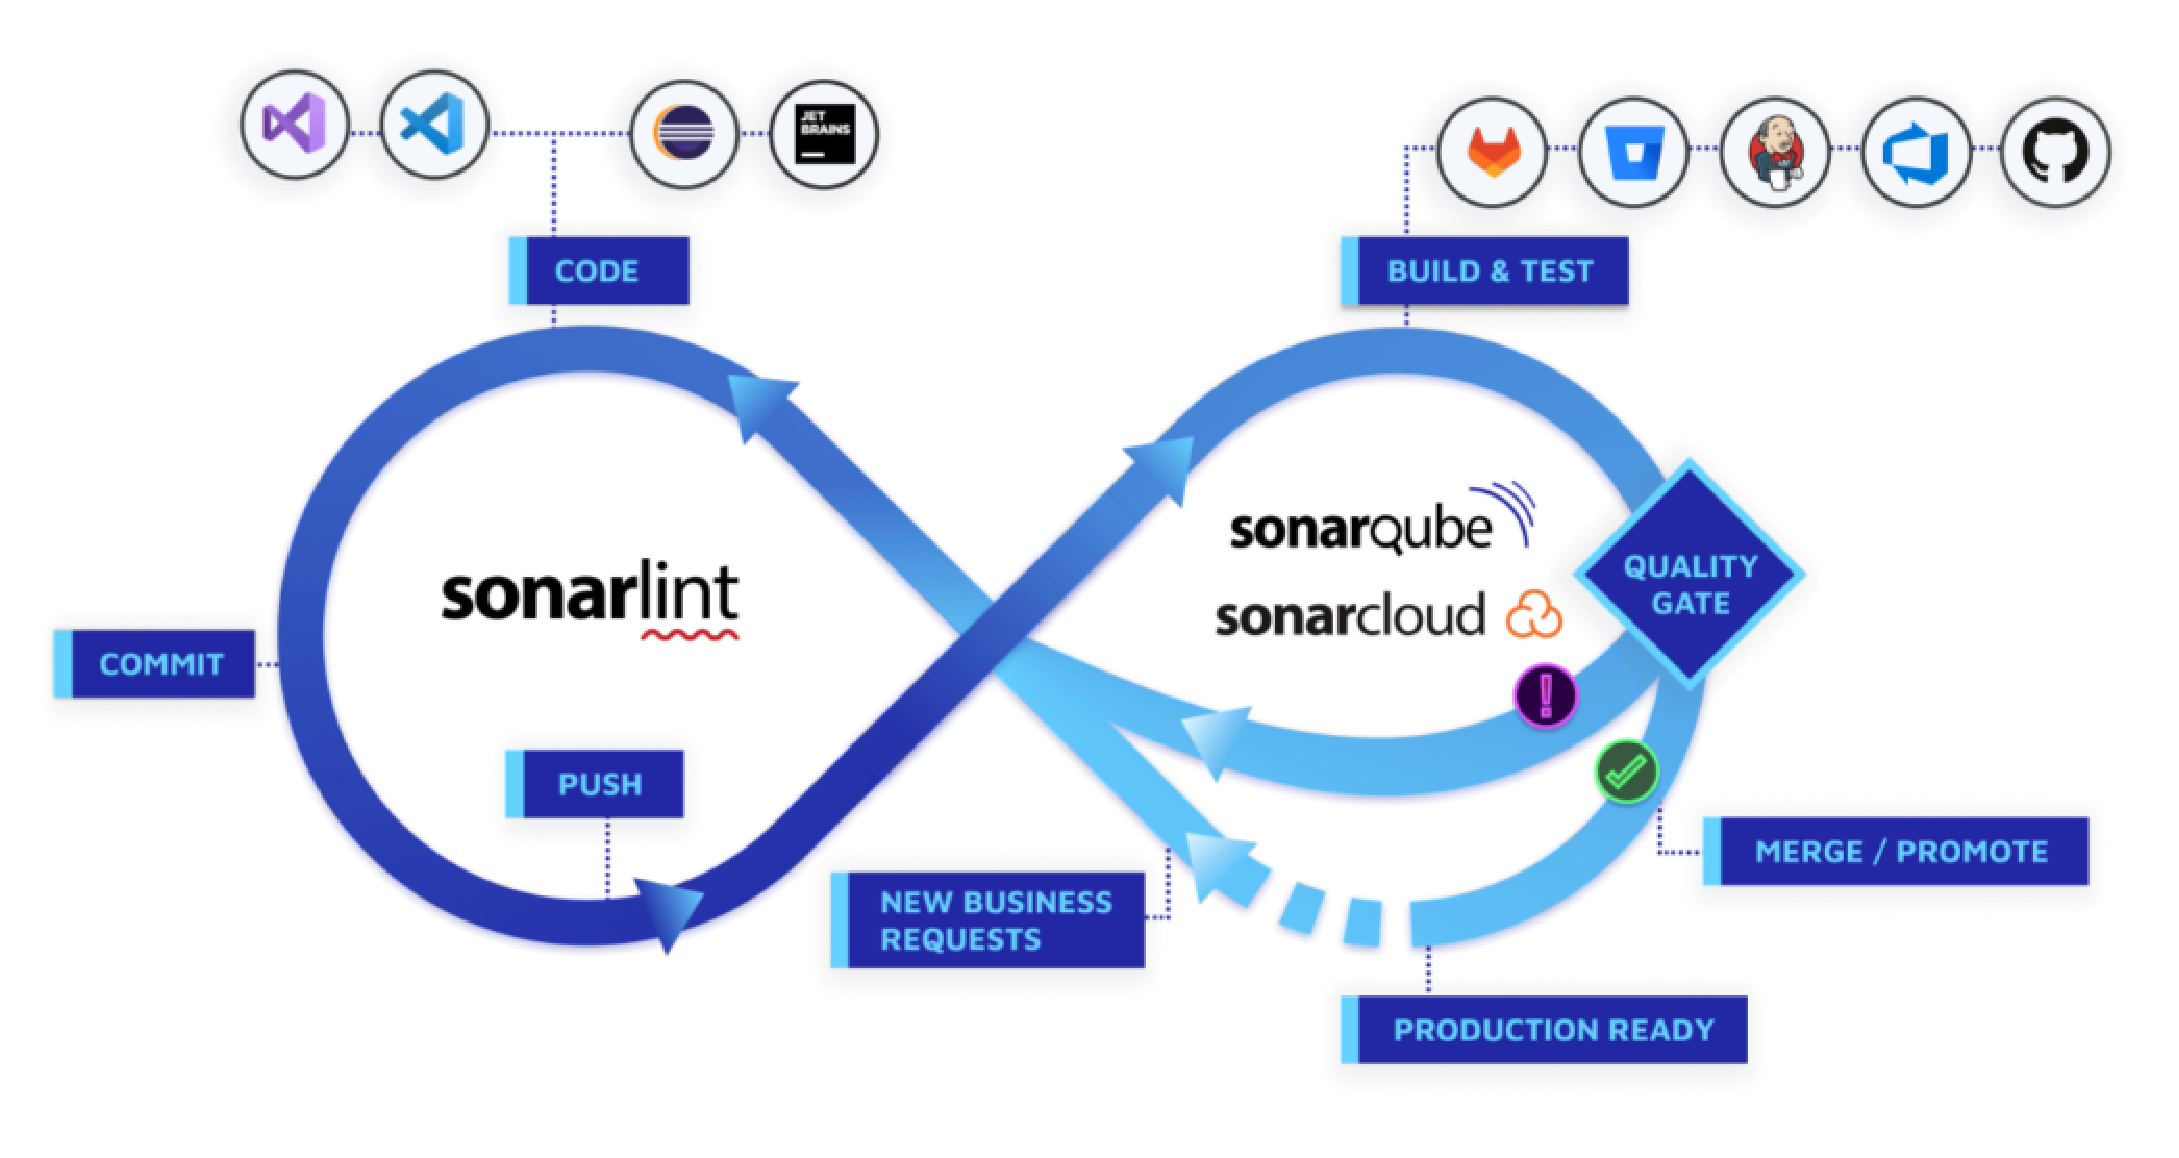
\includegraphics[keepaspectratio=true,scale=0.4]{figuras/sonarqube-workflow.eps}
    \parbox{\linewidth}{\centering FONTE: \cite{SonarQube}}
	\label{fig-sonarqube-workflow}
\end{figure}

Figura \ref{fig-sonarqube-workflow} demostra como o SonarQube pode ser utilizado no processo de desenvolvimento de \textit{software}. Esta ferramenta pode 
ser integrada ao CI/CD de um projeto a fim analisar os \textit{Pull Requests} criados, e com isso, toda nova submissão de 
código terá sua qualidade analisada. Com essa análise de \textit{Pull Requests}, é possível configurar um portão de qualidade, 
que, a partir de critérios de qualidade determinados, delimita se o código fonte submetido está de acordo com os padrões de \textit{Clean Code} 
e está apto a ir para produção, ou se ele deve voltar para a etapa de desenvolvimento.

A análise que o SonarQube realiza no projeto colabora muito com a avaliação de qualidade do mesmo. Com os dados fornecidos 
pela ferramenta, o time de desenvolvimento pode facilmente realizar correções no código a fim de aumentar sua qualidade, e 
também resolver possíveis vulnerabilidades presentes na implementação.

\section{Ferramentas de Apoio}

\subsection{GitHub}

O GitHub \footnote{https://github.com. Accesado pela última vez em 31/10/2023} é uma plataforma muito popular de hospedagem de projetos
de \textit{software} utilizando o Git \footnote{https://git-scm.com. Accesado pela última vez em 31/10/2023}, 
permitindo que desenvolvedores do mundo todo contribuam em projetos privados ou públicos. O Git 
é uma ferramenta de código livre e gratuita para versionamento de código fonte, que possui diversas funcionalidades 
para o desenvolvimento colaborativo de \textit{software}.

\subsection{Draw.io}

O Draw.io \footnote{https://www.drawio.com. Accesado pela última vez em 31/10/2023} é um \textit{software} online e grátis para a modelagem de diagramas. 
Esta ferramenta 
pode ser utilizada para criar os diversos tipos de diagramas presentes na \textit{Engenharia de Software}, 
como os diagramas UML, que são muito populares na fase de planejamento de produtos de \textit{software}.


\section{Considerações Finais do Capítulo}

Neste capítulo foram apresentadas as principais ferramentas de desenvolvimento e de apoio a serem utilizadas 
no desenvolvimento desse trabalho. A tabela \ref{tb:suportetecnologico} tem o objetivo de fornecer um 
resumo dos principais suportes tecnológicos.

\begin{table}[htb]
    \centering
    \caption{Suporte Tecnológico}
    \renewcommand{\arraystretch}{1.5}
    \begin{tabular}{p{2cm}p{5cm}p{1.5cm}p{5.5cm}}
        \toprule
        \textbf{Nome} & \textbf{Descrição}  & \textbf{Versão}  & \textbf{Link}  \\
        \midrule
        \rowcolor{gray!20} Node & \textit{Framework} para criação de APIs. & 20.9.0 & \url{https://nodejs.org/} \\
        Jest & \textit{Framework} para criação de testes automatizados. & 29.7.0 & \url{https://jestjs.io/} \\
        \rowcolor{gray!20} Docker & Ferramenta de virtualização de ambientes. & 24.0.0 & \url{https://www.docker.com/} \\
        Firebase & Conjuntos de serviços para desenvolvimento de aplicações em nuvem. & - & \url{https://firebase.google.com/} \\
        \rowcolor{gray!20} MongoDB & Banco de dados NoSQL para armazenamento de dados. & 7.0 & \url{https://www.mongodb.com/} \\
        SonarQube & Ferramenta de análise e controle de qualidade de código fonte. & 10.0 & \url{https://www.sonarsource.com/} \\
        \rowcolor{gray!20} GitHub & Plataforma de hospedagem de projetos de \textit{software}. & - & \url{https://github.com/} \\
        Draw.io & Ferramenta de modelagem de diagramas. & - & \url{https://www.drawio.com/} \\
        \bottomrule
    \end{tabular}
    \parbox{\linewidth}{\centering FONTE: Autores}
    \label{tb:suportetecnologico}
\end{table}
